\frame{\titlepage}

\begin{frame}
	Wer ist denn das?\absatz
	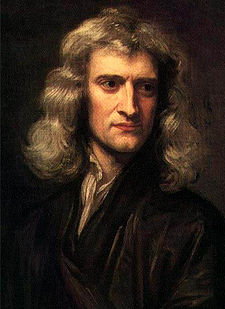
\includegraphics[width=0.25\textwidth]{img/newton.jpg}  \hfill 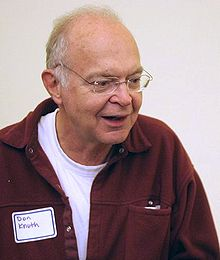
\includegraphics[width=0.25\textwidth]{img/knuth.jpg} \hfill \includegraphics[width=0.25\textwidth]{img/lamport.jpg}\\ \fabsatz
	Was haben sie miteinander zu tun?\\
	Was haben sie mit \LaTeX~zu tun?\\
	Was soll das ganze?
\end{frame}

\begin{frame}
	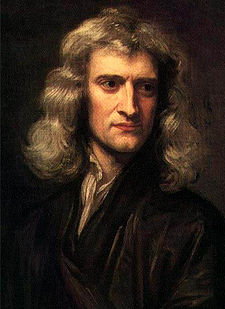
\includegraphics[width=0.25\textwidth]{img/newton.jpg} \hfill 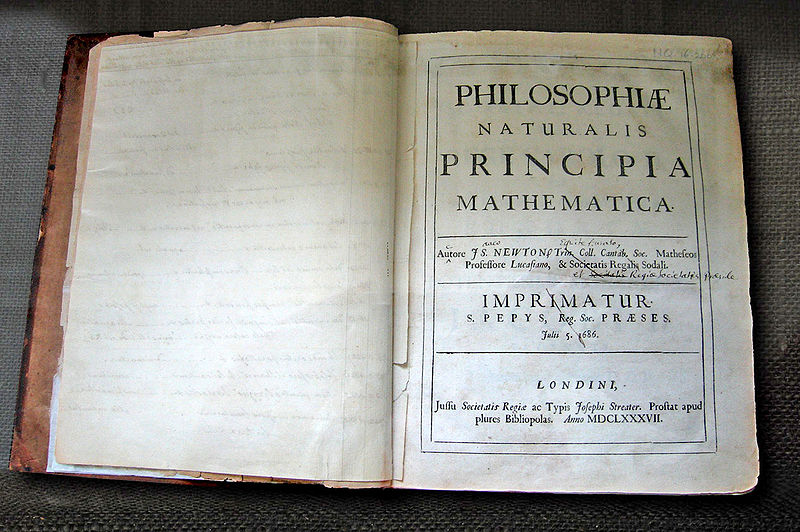
\includegraphics[width=0.25\textwidth]{img/Principia.jpg}\\\fabsatz
	Sir Isaac Newton
	\begin{itemize}
		\item * 1643 (in Woolsthorpe-by-Colsterworth)
		\item Naturforscher und Verwaltungsbeamter (wiki)
		\item Verfasser der {\sl Philosophiae Naturalis Principia Mathematica}
	\end{itemize}
\end{frame}

\begin{frame}
	
\includegraphics[width=1.00\textwidth]{img/newton_quote.png}
\end{frame}

\begin{frame}
	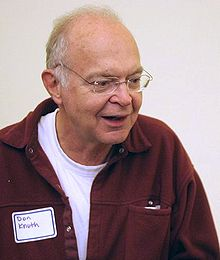
\includegraphics[width=0.25\textwidth]{img/knuth.jpg} \hfill 
\includegraphics[width=0.25\textwidth]{img/tAoCP.jpg}\\\fabsatz
	Don(ald Ervin) Knuth
	\begin{itemize}
		\item * 1938\\
		\item Prof. em. f\"u{}r Informatik an der Stanford U
		\item Verfasser von {\sl The Art of Computer Programming}
	\end{itemize}
\end{frame}

\begin{frame}
	\TeX\\
	\begin{itemize} 
		\item Entwicklung: 5. Mai 1977 -- 21. Mai 1986\\
		\item \small "`Ever since those beginnings in 1977, the \TeX~research project that I embarked on was driven by two major goals. The first goal was quality: we wanted to produce documents that were not just nice, but actually the best. [...] The second major goal was archival: to create systems that would be independent of changes in printing technology as much as possible. When the next generation of printing devices came along, I wanted to be able to retain the same quality already achieved, instead of having to solve all the problems anew. I wanted to design something that would be still usable in 100 years."' \\ \normalsize \phantom{a} \hfill Donald E. Knuth: Digital Typography
	\end{itemize}	
\end{frame}

\begin{frame}
	Warum \TeX?
	\begin{itemize}
		\item Komplexer Textsatz (Ligaturen, Formeln, ...)
		\pause
		\item Klare Formatierung durch Befehle
			\begin{itemize}
				\item Absturzsicherheit
				\item Wiederverwendbarkeit
			\end{itemize}
		\pause
		\item \TeX~\"ubernimmt (auf Wunsch) selbst die Organisation des Texts
		\pause
		\item \LaTeX~nimmt Arbeit ab:
			\begin{itemize}
				\item Nummerierungen aller Art
				\item Querverweise
				\item Formatierungen, die an mehreren Stellen vorkommen
				\item ...
			\end{itemize}
			\pause
		\item Sieht gut aus! (Das ist durchaus als Anspruch an die selbst produzierten Texte zu verstehen.)
	\end{itemize}
\end{frame}

\begin{frame}
	\includegraphics[width=0.25\textwidth]{img/lamport.jpg}\\\fabsatz
	Leslie Lamport
	\begin{itemize}
		\item * 1941
		\item Informatiker, zurzeit bei Microsoft Research
		\item \small "`In the early 80s, I was planning to write the Great American Concurrency Book.  I was a \TeX~user, so I would need a set of macros.  I thought that, with a little extra effort, I could make my macros usable by others."' 
		\pause \item "`[...]  Meanwhile, I still haven't written the Great American Concurrency Book."' \normalsize
	\end{itemize}
\end{frame}

\begin{frame}
	\LaTeX~ist ein benutzerfreundliche(re)s Textsatzsystem, das h\"a{}ufige Befehlsmakros zur Verf\"ugung stellt
	\begin{itemize}
		\item {\sl package}, dadurch
		\begin{itemize}
			\item erweiterbar
			\item personalisiert
		\end{itemize}
		\item werden von allen m\"oglichen Leuten auf der ganzen Welt geschrieben
		\item es gibt nichts was es nicht gibt:
			\begin{itemize}
				\item diese Pr\"asentation
				\item alle \"Ubungszettel, die ihr je in der Hand hattet
				\item ein Teil der offiziellen Briefe der Universit\"at
				\item Anteil von gesch\"atzt $> 70$\% der nat.-wiss. Fachb\"ucher
				\item ...
			\end{itemize}
	\end{itemize}
\end{frame}

\begin{frame}
	Was nicht stimmt:
	\pause
	\begin{itemize}
		\item \LaTeX~sei umst�ndlich (wenn es das ist, macht man was falsch!)
		\pause
		\item \LaTeX~sei perfekt (die {\sl package}s werden auch nur von Menschen geschrieben, wenn auch meist welchen mit viel Ahnung)
		\pause
		\item \TeX/\LaTeX~sei eine Programmiersprache (Textsatzsystem bzw. \"Uberbau dazu)
		\pause
		\item ein \LaTeX-Quelltext-File werde kompiliert (interpretiert, wenn \"uberhaupt; das alles hier hat nichts mit Maschinencode zu tun) $\longleftarrow$ das sagen wir aber trotzdem!
	\end{itemize}
	\pause
	... und bitte: X ist ein Chi ($\chi$)!
\end{frame}

\begin{frame}
	Auf geht's! Kursinhalte:
	\begin{itemize}
		\item Grundstrukturen von \TeX
		\item Mathematische Befehle (zum Teil \TeX, meist AMS-\LaTeX)
		\item Strukturen (Kapitel, Aufz\"ahlungen, ...) (\LaTeX)
		\item Elemente (Grafiken, Tabellen, ...) (\LaTeX)
		\item Hilfe zur Selbsthilfe!
	\end{itemize}
\end{frame}